\begin{problem}{뱀 수열}{standard input}{standard output}{3 seconds}{1024 megabytes}

2차원 평면 위에 $N$개의 사과가 놓여 있다.
한 마리의 뱀이 원점 $(0,\,0)$에서 출발하여, 이 중 일부를 골라 순서대로 먹으며 이동한다.

뱀의 출발점을 $P_0 = (0,\,0)$으로 놓고, 먹는 사과의 위치를 순서대로 $P_1, P_2, \ldots, P_L$이라 하자.

뱀은 \textbf{오른쪽 위}로만 전진한다.즉, 모든 $0 \leq i < L$에 대해 $x_i < x_{i+1}$이고 $y_i < y_{i+1}$이다. 각 점의 좌표를 $P_i = (x_i,\, y_i)$로 쓴다.

뱀은 \textbf{지그재그}로 나아간다.
연속한 두  사이의 이동 기울기를 $s_i = \dfrac{y_{i+1} - y_i}{x_{i+1} - x_i}$ ($0 \leq i < L$)라 정의하자.
$L \geq 2$일 때, 기울기 수열 $s_0, s_1, \ldots, s_{L-1}$은 다음 두 형태 중 하나를 만족해야 한다.

$$s_0 > s_1 < s_2 > s_3 < \cdots \quad \text{또는} \quad s_0 < s_1 > s_2 < s_3 > \cdots$$

\begin{center}
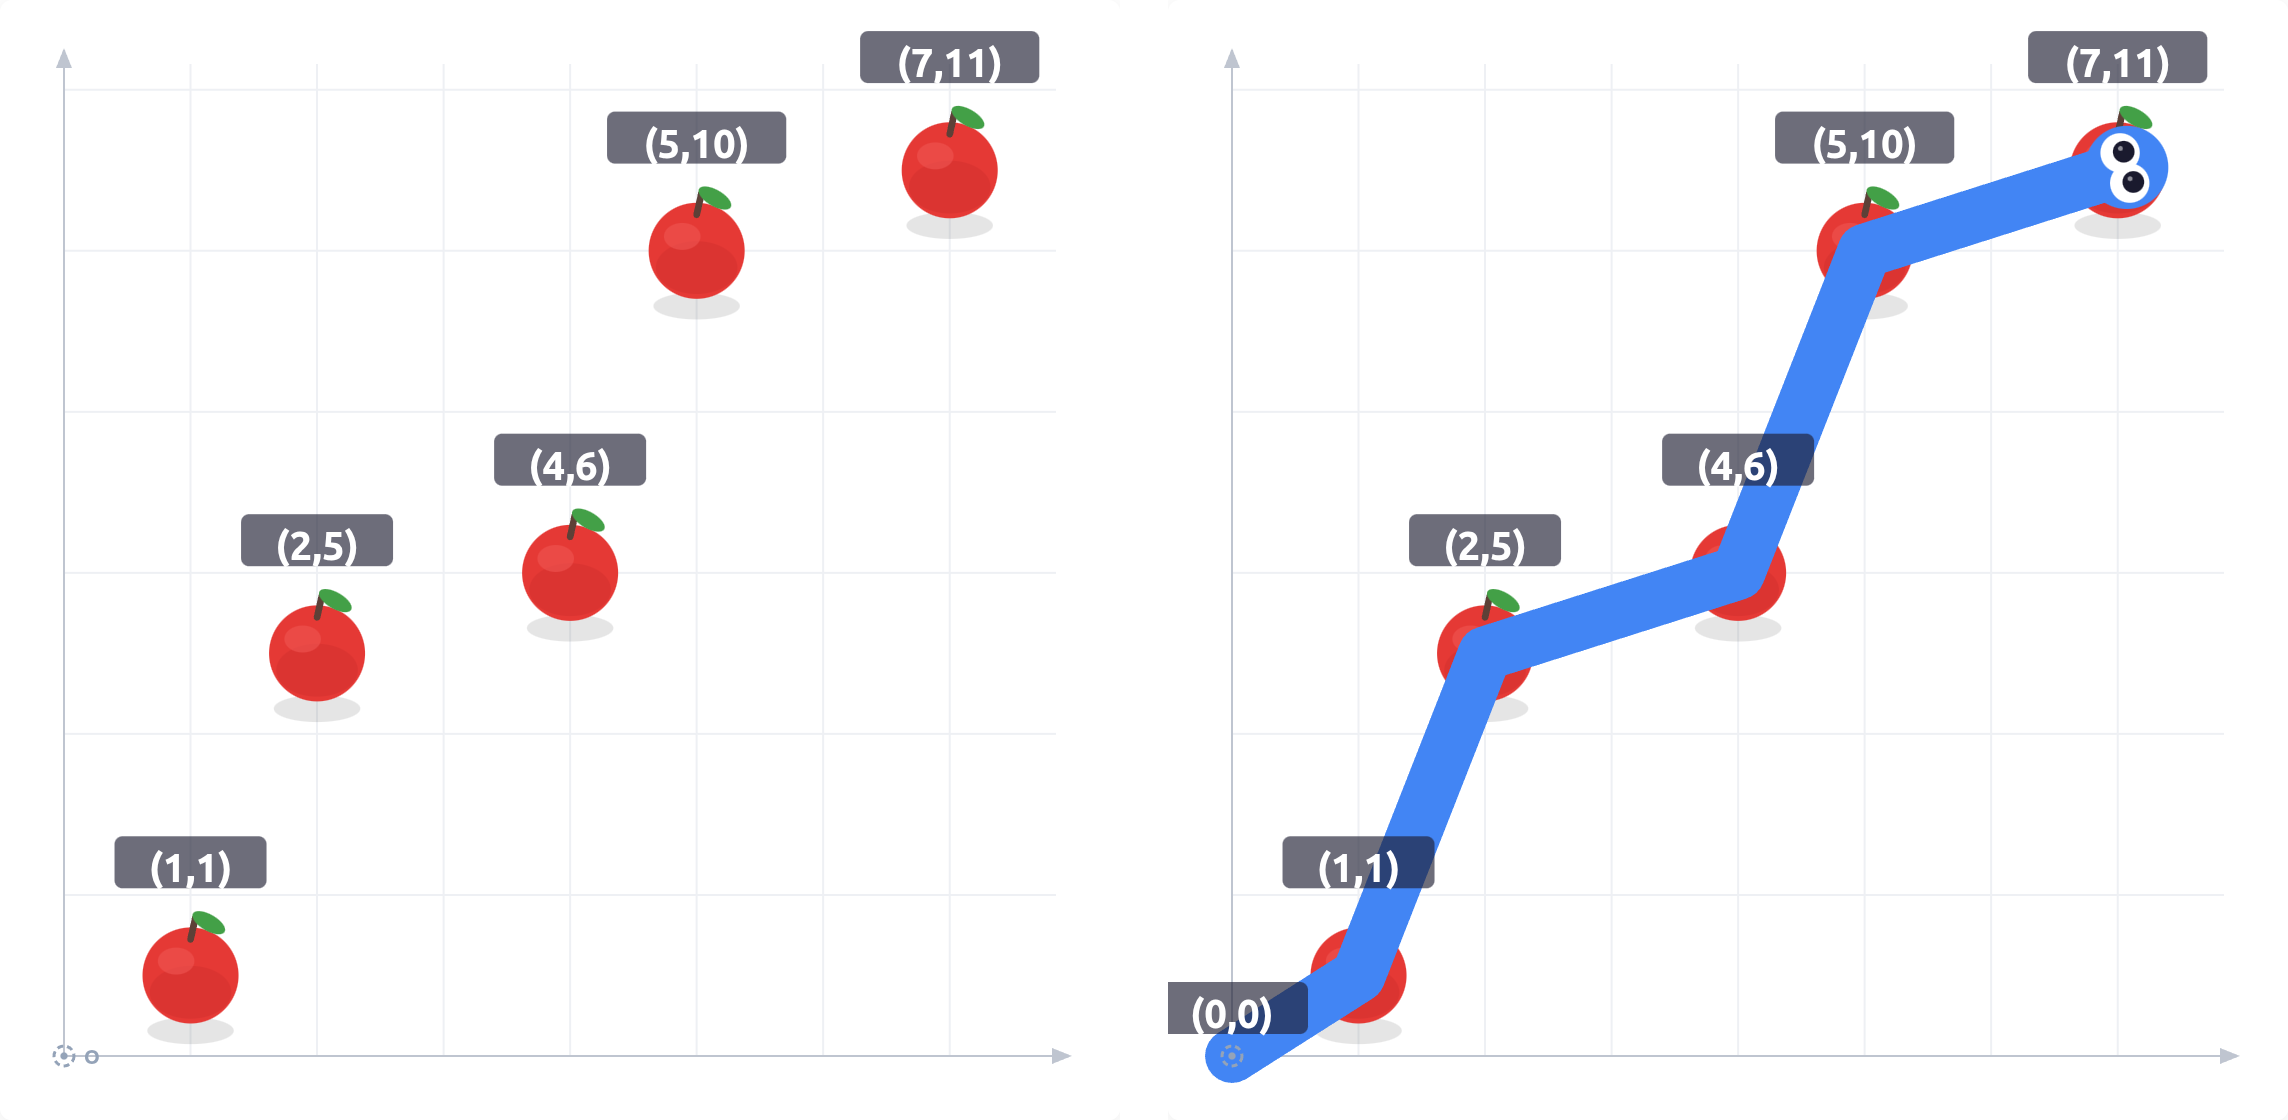
\includegraphics[width=16cm]{img.png}\\
{\small 예제 4의 사과 배치(왼쪽)와 최적 경로 $L = 5$(오른쪽)를 나타낸 것이다.}
\end{center}

뱀이 먹을 수 있는 사과의 최대 개수 $L$을 구하여라.

\InputFile
첫째 줄에 사과의 개수를 나타내는 정수 $N$이 주어진다.

다음 $N$개의 줄에 각각 사과의 $x$좌표와 $y$좌표를 의미하는 두 정수 $x$, $y$가 공백으로 구분되어 주어진다.

\OutputFile
뱀이 먹을 수 있는 사과의 최대 개수를 출력한다.

\Examples

\begin{example}
\exmpfile{example.01}{example.01.a}%
\exmpfile{example.02}{example.02.a}%
\exmpfile{example.03}{example.03.a}%
\exmpfile{example.04}{example.04.a}%
\end{example}

\end{problem}

